\documentclass[
	spanish,
]{beamer}

% ====================================
% Packages & Style
% ====================================

\usepackage{Personal}
\usetheme{Madrid}
\setbeamertemplate{navigation symbols}{}
\setbeamercovered{transparent}
% \setbeamertemplate{footline}{}
\usetikzlibrary{external}
\tikzexternalize[prefix=__cache__/]



% ====================================
% Bibliografía
% ====================================

\usepackage[
  backend=biber,
  defernumbers=true,
  style=numeric
]{biblatex}
\addbibresource{Contenido/B-Bibliografia/bibliografia.bib}
\usepackage{hyperref}

% ====================================
% Portada
% ====================================

\title[Cálculo de Geodésicas en $\mathbb{H}^{2}$]{Cálculo de Geodésicas en el Espacio Hiperbólico de Dimensión 2}
\author[Ángel Peñaflor]{
	Ángel Emmanuel Peñaflor Zetina \\[12pt]
	\footnotesize Directores: \\
	Dr. Francisco Gabriel Hernández Zamora \\
	Dr. Evodio Muñoz Aguirre
}
\institute[UV]{Universidad Veracruzana \\ Facultad de Matemáticas}

% ====================================
% Documento
% ====================================

\begin{document}

\maketitle

\begin{frame}
\frametitle{Introducción}
  \begin{block}{Objetivo}
    Encontrar las curvas geodésicas en el espacio hiperbólico de dimensión 2.
  \end{block} \pause

  \begin{itemize}
    \item ¿Qué es una curva geodésica? \pause
    \item ¿Qué es el espacio hiperbólico de dimensión 2? 
  \end{itemize}
\end{frame}

\begin{frame}
\frametitle{Variedades Topológicas}
\begin{definition}[Variedad Topológica]
  Sea $M$ un espacio topológico, diremos que $M$ es una \textbf{variedad topológica de dimensión $n$} si:
  \begin{itemize}
    \item $M$ es un \textit{espacio de Hausdorff}.
    \item $M$ es \textit{segundo numerable}.
    \item $M$ es \textit{localmente euclidiano de dimensión $n$}, esto quiere decir que, para cada punto $x \in M$ existe una vecindad abierta $U$ que contiene a $x$ y un homeomorfismo $\phi: U \to \phi(U)\subseteq \R^n$.
  \end{itemize}
\end{definition}
\end{frame}

\begin{frame}
\centering
\begin{figure}
  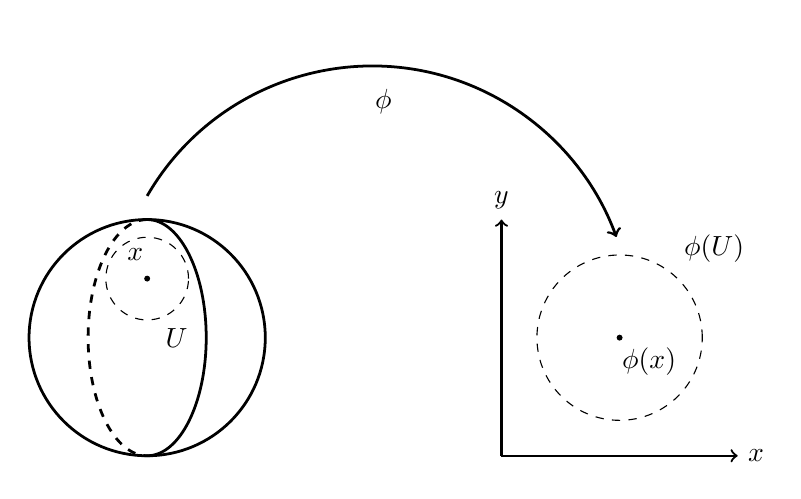
\begin{tikzpicture}[scale=1.5]
  \draw[line width=1] (-3,2) arc (90:-90:0.5 and 1);
  \draw[line width=1, dashed] (-3,2) arc (90:270:0.5 and 1);
  \draw[line width=1](-3,1) circle (1);
  \draw[color=black,thick,->] (0,0) -- (2,0) node[anchor=west]{$x$};
  \draw[color=black,thick,->] (0,0) -- (0,2) node[anchor=south]{$y$};

  \filldraw[black] (1,1) circle (0.02);
  \draw[dashed] (1,1) circle (0.7);
  \draw node at (1.25,0.80) {$\phi(x)$};
  \draw node at (1.8,1.75) {$\phi(U)$};

  \filldraw[black] (-3,1.5) circle (0.02);
  \draw node at (-3.1,1.70) {$x$};
  \draw[dashed] (-3,1.5) circle (0.35);
  \draw node at (-2.75,1) {$U$};

  \draw[line width=1, ->] (-3,2.2) arc (150:20:2.2);
  \draw node at (-1,3) {$\phi$};
\end{tikzpicture}

  \caption{Ejemplo de un homeomorfismo de una variedad a $\R^{2}$.}
\end{figure}
\end{frame}

\begin{frame}
\frametitle{Ejemplo de Variedades Topológicas}
\begin{columns}[t]
\column{.5\textwidth}
\centering
  \begin{figure}
    \scalebox{.5}{\tdplotsetmaincoords{70}{135}
\begin{tikzpicture}[scale=3,line join=bevel,tdplot_main_coords]
{\draw[color=black,thick,->] (0,0,0) -- (1,0,0) node[anchor=north east]{$x$};}%
{\draw[color=black,thick,->] (0,0,0) -- (0,1,0) node[anchor=north west]{$y$};}%
{\draw[color=black,thick,->] (0,0,0) -- (0,0,1) node[anchor=south]{$z$};}%
\end{tikzpicture}
}\\
    \caption{Los Espacios Euclidianos, $\R^n$.}
  \end{figure}
  \begin{figure}
    \scalebox{.5}{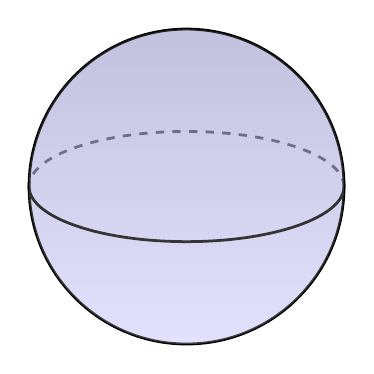
\begin{tikzpicture}[scale=2]
  \draw[line width=1, dashed] (1,0) arc (0:180:1 and 0.35);
  \draw[fill=blue!30!white!,opacity=0.5] (0,0) circle (1);
  \draw[line width=1] (1,0) arc (0:180:1 and -0.35);
  \draw[line width=1](0,0) circle (1);
  \shade[opacity=0.25] (0,0) circle (1);
\end{tikzpicture}

}\\
  \caption{La $n-$esferas, $\S^n$.}
  \end{figure}
\column{.5\textwidth}
\centering
  \begin{figure}
    \scalebox{.5}{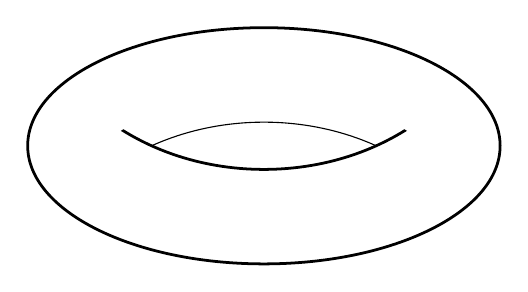
\begin{tikzpicture}
  \useasboundingbox (-3,-1.5) rectangle (3,1.5);
  \draw[line width=1] (0,0) ellipse (3 and 1.5);
  \begin{scope}
    \clip (0,-1.8) ellipse (3 and 2.5);
    \draw[line width=1] (0,2.2) ellipse (3 and 2.5);
  \end{scope}
  \begin{scope}
    \clip (0,2.2) ellipse (3 and 2.5);
    \draw (0,-2.2) ellipse (3 and 2.5);
  \end{scope}
\end{tikzpicture}
}\\
    \caption{El $n-$Toro, $\mathbb{T}^n$.}
  \end{figure}
  \begin{figure}
    \centering
    \scalebox{.5}{\begin{tikzpicture}[scale=4.5]
{\draw[color=black,thick,->] (0,0) -- (1,0) node[anchor=west]{$x$};}%
{\draw[color=black,thick,->] (0,0) -- (0,1) node[anchor=south]{$y$};}%
\draw[dashed] (0.5,0.5) circle (0.25);
\filldraw[black] (0.5,0.5) circle (0.02);
\end{tikzpicture}
}\\
    \caption{Los subconjuntos abiertos\\ de las variedades.}
  \end{figure}
\end{columns}
\end{frame}

\begin{frame}
\frametitle{Ejemplo: El Espacio Proyectivo}
\centering
\begin{figure}
  \scalebox{0.75}{\begin{tikzpicture}[scale=1.75]
\draw[color=black] (-2,0) -- (2,0);
\draw[color=black] (0,-2) -- (0,2);
\draw[thick] (0,0) circle (1);
\draw[thick] (-1.5, -1.5) -- (1.5,1.5); 
\filldraw[red] (0.71,0.71) circle (0.04);
\filldraw[blue] (-0.71,-0.71) circle (0.04);
\end{tikzpicture}
}
  \caption{Representación del Espacio Proyectivo $\mathbb{RP}^{2}$.}
.\end{figure}
\end{frame}

\begin{frame}
\frametitle{Cartas}
\begin{definition}[Carta]
  Una \textbf{carta} en $M$ es un par ordenado $(U,\phi)$ donde $U$ es un subconjunto abierto de $M$ y $\phi$ es un homeomorfismo de $U$ a $\R^n$.
\end{definition}\pause

\begin{definition}[Cartas Suavemente Compatibles]
  Si $(U,\phi)$ y $(V,\psi)$ son dos cartas en $M$ tales que $U \cap V \neq \varnothing$, llamaremos \textbf{mapa de transición} a la composición de funciones:
  \[ \psi \circ \phi^{-1}: \phi(U \cap V) \to \psi(U \cap V) \]
  
  Y además diremos que las cartas $(U,\phi)$ y $(V,\psi)$ son \textbf{suavemente compatibles} si $U \cap V = \varnothing$ o si el mapa de transición $\psi \circ \phi^{-1}$ es un difeomorfismo.
\end{definition}
\end{frame}

\begin{frame}
  \centering
  \begin{figure}
    \begin{tikzpicture}[scale=1]
	\coordinate (a) at (0,0);
	\path[draw,use Hobby shortcut,closed=true,thick]
	(0,2.5) .. (2,2.5) .. (1,4.5) .. (.3,4.5) .. (-1,4) .. (-2,2.5);

	\begin{scope}
		\clip (0.25,3.5) circle (0.5);
		\fill[blue!30!white,opacity=0.5] (-0.25,3.25) circle (0.5);
	\end{scope}
	\draw[dashed] (0.25,3.5) circle (0.5);
	\draw[dashed] (-0.25,3.25) circle (0.5);
	\draw node at (0.8,4) {$V$};
	\draw node at (-0.9,2.75) {$U$};

	\draw [thick, <->] (-5,0) -- (-1,0);
	\draw [thick, <->] (-3,-2) -- (-3,2);
	\draw [thick, <->] (1,0) -- (5,0);
	\draw [thick, <->] (3,-2) -- (3,2);

	\begin{scope}
		\clip (-3,0.5) ellipse  (0.8 and 1);
    \fill[color=blue!30!white,opacity=0.5] (-2.5,0) ellipse  (1.2 and 0.8);
	\end{scope}
	\draw [dashed,thick] (-3,0.5) ellipse  (0.8 and 1);
	% \draw [dashed,thick] (-2.5,0) ellipse  (1.2 and 0.8);

	\begin{scope}
		\clip (3,0.5) ellipse  (0.8 and 1);
		\fill[color=blue!30!white,opacity=0.5](3.5,0) ellipse  (1.2 and 0.8);
	\end{scope}
	% \draw [dashed,thick] (3,0.5) ellipse  (0.8 and 1);
	\draw [dashed,thick] (3.5,0) ellipse  (1.2 and 0.8);

	\draw[line width=1, ->] (1,3.75) arc (90:-5:2.5);
	\draw[line width=1, ->] (-1,3.25) arc (-90:0:-1.5);
	\draw[line width=1, ->] (-1.75,0.5) -- (2,0.5);

	\draw node at (-2.5,2.75) {$\phi$};
	\draw node at (3.25,3) {$\psi$};
	\draw node at (-4.25,1.25) {$\phi(U)$};
	\draw node at (4.5,1) {$\psi(V)$};
	\draw node at (0.25,1) {$\psi \circ \phi^{-1}$};


\end{tikzpicture}
  
    \caption{Mapa de Transición}
  \end{figure}
\end{frame}

\begin{frame}
  \frametitle{Atlas y la Estructura Suave}
  \begin{definition}[Atlas, Atlas Suave y Atlas Maximal]
    \begin{itemize}
      \item Una colección de cartas $(U,\phi)_{\alpha}$ es un \textbf{atlas} $\mathcal{A}$, en $M$ si dichas cartas forman una cubierta para $M$.
      \item Diremos que el atlas $\mathcal{A}$ es \textbf{suave} si cualesquiera dos cartas son suavemente compatibles, a las cartas de un atlas suaves les llamaremos \textit{cartas suaves}.
      \item Un atlas suave es llamado \textbf{maximal} si no está propiamente contenido en ningún atlas más grande.
    \end{itemize}
  \end{definition}\pause

  \begin{definition}[Variedad Suave]
    Si $M$ es una variedad topológica y $\mathcal{A}$ es un atlas maximal en $M$, diremos que el par $(M,\mathcal{A})$ es una \textbf{variedad suave}, a dicho atlas maximal le llamaremos la \textbf{estructura suave} en $M$.
  \end{definition}
\end{frame}


\begin{frame}
\frametitle{Ejemplo de Variedades Suaves}
\begin{columns}[t]
\column{.5\textwidth}
\centering
  \begin{figure}
    \scalebox{.5}{\tdplotsetmaincoords{70}{135}
\begin{tikzpicture}[scale=3,line join=bevel,tdplot_main_coords]
{\draw[color=black,thick,->] (0,0,0) -- (1,0,0) node[anchor=north east]{$x$};}%
{\draw[color=black,thick,->] (0,0,0) -- (0,1,0) node[anchor=north west]{$y$};}%
{\draw[color=black,thick,->] (0,0,0) -- (0,0,1) node[anchor=south]{$z$};}%
\end{tikzpicture}
}\\
    \caption{Los Espacios Euclidianos, $\R^n$.}
  \end{figure}
  \begin{figure}
    \scalebox{.5}{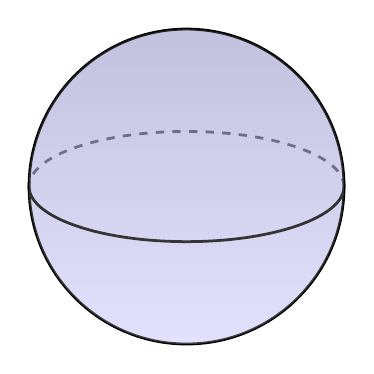
\begin{tikzpicture}[scale=2]
  \draw[line width=1, dashed] (1,0) arc (0:180:1 and 0.35);
  \draw[fill=blue!30!white!,opacity=0.5] (0,0) circle (1);
  \draw[line width=1] (1,0) arc (0:180:1 and -0.35);
  \draw[line width=1](0,0) circle (1);
  \shade[opacity=0.25] (0,0) circle (1);
\end{tikzpicture}

}\\
  \caption{La $n-$esferas, $\S^n$.}
  \end{figure}
\column{.5\textwidth}
\centering
  \begin{figure}
    \scalebox{.5}{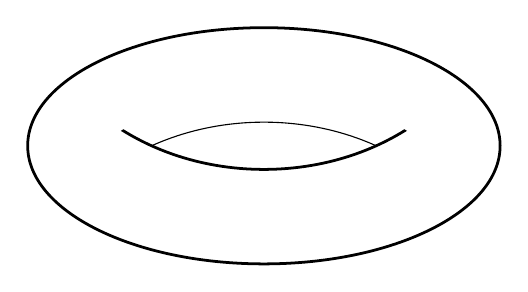
\begin{tikzpicture}
  \useasboundingbox (-3,-1.5) rectangle (3,1.5);
  \draw[line width=1] (0,0) ellipse (3 and 1.5);
  \begin{scope}
    \clip (0,-1.8) ellipse (3 and 2.5);
    \draw[line width=1] (0,2.2) ellipse (3 and 2.5);
  \end{scope}
  \begin{scope}
    \clip (0,2.2) ellipse (3 and 2.5);
    \draw (0,-2.2) ellipse (3 and 2.5);
  \end{scope}
\end{tikzpicture}
}\\
    \caption{El $n-$Toro, $\mathbb{T}^n$.}
  \end{figure}
  \begin{figure}
    \centering
    \scalebox{.5}{\begin{tikzpicture}[scale=4.5]
{\draw[color=black,thick,->] (0,0) -- (1,0) node[anchor=west]{$x$};}%
{\draw[color=black,thick,->] (0,0) -- (0,1) node[anchor=south]{$y$};}%
\draw[dashed] (0.5,0.5) circle (0.25);
\filldraw[black] (0.5,0.5) circle (0.02);
\end{tikzpicture}
}\\
    \caption{Subconjuntos abiertos\\ de variedades suaves.}
  \end{figure}
\end{columns}
\end{frame}

\begin{frame}
\begin{definition}[Función Suave \textbf{Incorrecta}]
  Sea $M$ una variedad topológica $n-$dimensional, $k$ un entero positivo y $f: M \to \R^{k}$ una función cualquiera, diremos que la función $f$ es suave si para cada carta $(U,\phi)$ se tiene que la composición $f \circ \phi^{-1}: \phi(U) \subseteq \R^n \to \R^k$ es diferenciable
\end{definition} \pause

\vspace{12pt}
\centering
Consideremos los siguientes atlas suaves en $\R$: 
\begin{columns}[t]
  \column{.5\textwidth}
  \begin{tcolorbox}[height=45pt]
    \centering
    \vspace{5pt}
    $(\R, \id_{\R})$
  \end{tcolorbox}
  \column{.5\textwidth}
  \begin{tcolorbox}[height=45pt]
    \centering
    $(\R, \psi)$,\\
    $\psi(x) = x^3$
  \end{tcolorbox}
  \centering
\end{columns} \pause

  \begin{tcolorbox}[width=0.3\linewidth, colframe=red]
  \centering
  $ \id_{\R} \circ \psi^{-1}(y) = y^{\frac{1}{3}}$
  \end{tcolorbox}
\end{frame}

\begin{frame}
  \frametitle{Funciones Suaves}
  \begin{definition}[Función Suave]
    Sean $M$ una variedad suave  $n-$dimensional, $k$ un entero no negativo y $f: M \to \R^{k}$ una función cualquiera. Diremos que $f$ es una \textbf{función suave} si para cada punto $p \in M$ existe una carta suave $(U,\phi)$, cuyo dominio contiene a $p$ y tal que la composición de funciones $f \circ \phi^{-1}$ es suave en el conjunto abierto $\phi(U) \subseteq \R^{n}$.
  \end{definition} \pause

  Notemos que esta definición coincide con la definición usual de diferenciabilidad cuando $M = \R^n$.
\end{frame}

\begin{frame}
  \begin{figure}
    \begin{tikzpicture}[scale=0.85]
  \coordinate (a) at (0,0);
\path[draw,use Hobby shortcut,closed=true,thick]
(0,2.5) .. (2,2.5) .. (1,4.5) .. (.3,4.5) .. (-1,4) .. (-2,2.5);

\draw[dashed] (0.25,3.5) circle (0.6);
\draw node at (0,3.6) {$U$};
\draw node at (-1.5,4.5) {$M$};

\draw [thick, <->] (-5,0) -- (-1,0);
\draw [thick, <->] (-3,-2) -- (-3,2);
\draw [thick, <->] (1,0) -- (5,0);
\draw [thick, <->] (3,-2) -- (3,2);

\draw [dashed,thick] (-3,-0.25) ellipse  (1.5 and 1.2);


\draw[line width=1, ->] (1,3.75) arc (90:0:2.5);
\draw[line width=1, ->] (-0.75,3.5) arc (-90:0:-2);
\draw[line width=1, ->] (-1.5,-1.5) arc (60:120:-3.5);

\draw node at (-2.75,3) {$\phi$};
\draw node at (3.25,3) {$f$};
\draw node at (-2.25,-0.5) {$\phi(U)$};
\draw node at (-4.5,1) {$\R^n$};
\draw node at (4.5,1) {$\R^{k}$};
\draw node at (0.5,-1.25) {$f \circ \phi^{-1}$};
\end{tikzpicture}

    \caption{Representación de una función suave.}
  \end{figure}
\end{frame}

\begin{frame}
\frametitle{Mapas Suaves}
  De modo similar, podemos definir los mapas suaves explotando el hecho de que sabemos cuando una función que va de $\R^m$ a $\R^n$ es suave. \pause

\begin{definition}[Mapa Suave]
  Sean $M$ y $N$ variedades suaves, $F: M \to N$ un mapa cualquiera. Diremos que $F$ es un \textbf{mapa suave} si para cada $p \in M$ existen cartas $(U,\varphi)$ que contiene a $p$ y $(V,\psi)$ que contiene a $F(p)$ tal que $F(U)\subset V$ y la composición $\psi \circ F \circ \varphi^{-1}$ es suave de $\varphi(U)$ a $\psi(V)$.
\end{definition}
\end{frame}

\begin{frame}
  \begin{figure}
    \scalebox{.70}{\begin{tikzpicture}[scale=1]

%Variedad M
\path[draw,use Hobby shortcut,closed=true]
(-5,5.5) .. (-6,4) .. (-4,4) .. (-2,3.5) .. (-2.5,6);
\filldraw (-3,5) circle (0.05);
\node at (-3.25,5.25) {$p$};
\node at (-2.25,4.35) {$U$};
\draw[dashed] (-3,5) ellipse (0.6 and 0.8);
\node at (-1.25,5.75) {$M$};

%Variedad N
\path[draw,use Hobby shortcut,closed=true]
(5.5,6) .. (6,4) .. (4,3) .. (2,3.5) .. (2.5,5) .. (3.5,5.5);
\filldraw (3.25,4) circle (0.05);
\node at (2.75,3.6) {$F(p)$};
\node at (4.25,5) {$V$};
\draw[dashed](3.25,4) ellipse (1.2 and 0.9);
\node at (2,5.25) {$N$};

% Flecha M a N
\draw[thick,->] (-1,6) arc (-60:-130:-2.5);
\node at (0.25,6.75) {$F$};

% Flecha M a Rm
\draw[thick,->] (-3,4) arc (-10:20:-5);
\node at (-3.5,2.75) {$\phi$};

% Flecha N a Rn
\draw[thick,->] (3.75,3.25) arc (10:-20:4);
\node at (4.25,2) {$\psi$};

%Eje Izquierdo
\draw [<->] (-5,-1) -- (-1,-1);
\draw [<->] (-4,-1.5) -- (-4,2.5);
\node at (-5,2.5) {$\R^m$};
\node at (-1,1.25) {$\phi(U)$};
\draw[dashed] (-2.5, 0.25) circle (1);

%Eje Derecho
\draw [<->] (5,-1) -- (1,-1);
\draw [<->] (2,-1.5) -- (2,2.5);
\node at (1,2.5) {$\R^n$};
\node at (4.5,0) {$\psi(V)$};
\draw[dashed] (2.5, -0.25) circle (1.2);

% Flecha Rn a Rm
\draw[thick,->] (-2,-1.25) arc (60:120:-3.5);
\node at (0,-2) {$\psi \circ F \circ \psi^{-1}$};
\end{tikzpicture}
}
    \caption{Representación de un mapa suave.}
  \end{figure}
\end{frame}

\begin{frame}
\frametitle{Ejemplo de Funciones y Mapas Suaves}
  \begin{itemize}
    \item Las mapas constantes.
    \item El mapa identidad.
    \item El mapeo de inclusión
    \item Composición de funciones suaves.
    \item Las proyecciones.
    \item Toda función $f: \R^m \to \R^n$ que sea suave en el sentido de usual del cálculo será también un mapa suave en el sentido de variedades.
  \end{itemize}
\end{frame}

\section{Espacios Tangentes}
\begin{frame}
	\frametitle{Espacios tangentes en $\R^n$}
	\begin{definition}[Vectores y Espacios Tangentes en $\R^n$]\label{Definición: Espacio Tangente en Rn}
		Sea $a$ un punto en $\R^n$, definiremos el \textbf{espacio tangente a $\R^n$ en el punto $a$} como el conjunto:
		\[ T_{a}(\mathbb{R}^{n}) = \{a\} \times \R^n = \{(a,v): v \in \R^n\} \]

		Un \bf{vector tangente} a $\R^n$ es un elemento de $T_a(\R^n)$ para algún $a \in \R^n$.
	\end{definition}\pause

	$T_a(\R^n)$ tiene estructura de espacio vectorial. Dados $a \in \mathbb{R}^{n}$, $c \in \mathbb{R}$ y $v_a, w_a \in T_a(\mathbb{R}^n)$:
	\begin{align*}
		v_a + w_a & = (v+w)_a \\
		c(v_a)    & = (cv)_a
	\end{align*}
\end{frame}

\begin{frame}
	\frametitle{Ejemplo de espacios tangentes}
	\begin{columns}[t]
		\column{.5\textwidth}
		\centering
		\begin{figure}
			\vspace{-12pt}
			\scalebox{.4}{\begin{tikzpicture}
\draw[thick,->] (-0.5,0) -- (5,0) node[anchor=west]{$x$};
\draw[thick,->] (0,-0.5) -- (0,5) node[anchor=south]{$y$};

\draw (0.5,0.5) rectangle (4,4);
\node at (4.5,4.5) {$T_a(\R^n)$};

\draw[thick,->] (1,1.5) -- (3.5,1.5);
\draw[thick,->] (1.5,1) -- (1.5,3.5);
\filldraw (1.5,1.5) circle (0.1);
\node at (1,1) {$a$};
\draw[thick, ->] (1.5,1.5) -- (3,2.75);
  \node at (3.25,2.5) {$v_a$};
\end{tikzpicture}

}\\
			\caption{Espacio tangente a un punto \\ en el plano.}
		\end{figure}
		\begin{figure}
			\vspace{-12pt}
			\scalebox{.4}{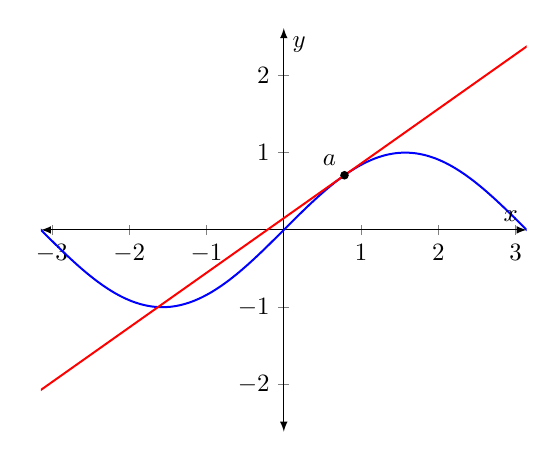
\begin{tikzpicture}[scale=0.90]
	\begin{axis}[
			% grid=both,
			xmin=-pi,
			xmax=pi,
			ymin=-1.6,
			ymax=1.6,
			axis lines=middle,
			xlabel = $x$,
			ylabel = $y$,
			axis line style={latex-latex},
      axis equal,
		]

		\addplot[
			samples=200,
			domain=-4*pi:4*pi,
			color=blue,
			thick,
			smooth,
		]
		{sin(deg(x))};

		\addplot[
			domain=-5:5,
			color=red,
      thick,
		]{( (sqrt(2) / 2) * (x - (pi/4)) ) +  (sqrt(2) / 2)};

		\addplot+[
			mark options={black},
      mark size=1.5pt,
		] coordinates {(0.785398,0.707106)} node [black, left=6pt, above=0.5pt] {$a$};
	\end{axis}
\end{tikzpicture}

}\\
			\caption{Espacio tangente a un punto \\ de $\sin(x)$.}
		\end{figure}
		\column{.5\textwidth}
		\centering
		\begin{figure}
			\scalebox{.5}{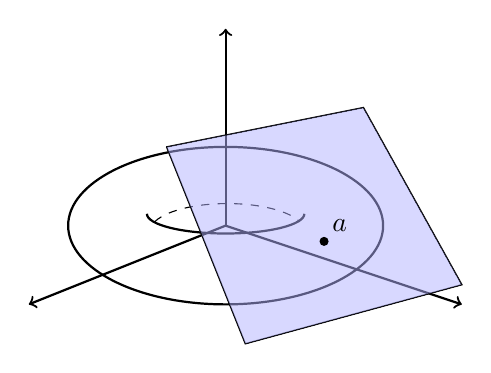
\begin{tikzpicture}

	% Ejes R3
	\draw [thick,->] (0,0) -- (0,2.5);
	\draw [thick,->] (0,0) -- (3,-1);
	\draw [thick,->] (0,0) -- (-2.5,-1);

	% Toro
	\draw [thick] (0,0) ellipse  (2 and 1);
	\draw [thick] (-1.0,0.15) arc (0:-180:-1.0 and 0.25);
  \draw [dashed] (-0.90,0.05) arc (20:160:-0.98 and 0.35);

  % Plano tangente
  \draw [line width=0.5] (-0.75,1) -- (1.75,1.5) -- (3,-0.75) -- (0.25,-1.5) -- (-0.75,1);
  \draw [fill=blue!30!white,opacity=0.5, line width=0] (-0.75,1) -- (1.75,1.5) -- (3,-0.75) -- (0.25,-1.5) -- (-0.75,1);

  % Punto $a$
	\filldraw (1.25,-0.2) circle (0.05);
	\node at (1.45,0) {$a$};
\end{tikzpicture}
}\\
			\caption{Espacio tangente a un punto \\ del $2-$toro.}
		\end{figure}
		\begin{figure}
			\vspace{-12pt}
			\scalebox{.45}{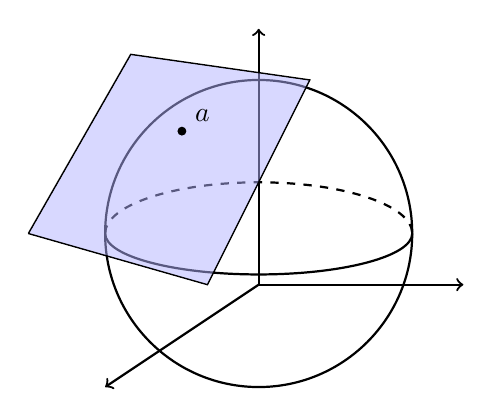
\begin{tikzpicture}[scale=0.65]
	% Esfera
	\draw [thick] (3,0) arc (0:180:3 and -0.8);
	\draw [thick, dashed] (-3,0) arc (180:0:3 and 1);
	\draw [thick] (0,0) circle (3);

	% Ejes R3
	\draw [thick,->] (0,-1) -- (0,4);
	\draw [thick,->] (0,-1) -- (4,-1);
	\draw [thick,->] (0,-1) -- (-3,-3);


	% Rectángulo (Espacio Tangente)
  \draw [fill=blue!30!white,opacity=0.5, line width=0] (-4.5,0) -- (-2.5,3.5) --(1,3.0) -- (-1,-1) -- (-4.5,0);
  \draw [line width=0.5] (-4.5,0) -- (-2.5,3.5) --(1,3.0) -- (-1,-1) -- (-4.5,0);
	\filldraw (-1.5,2) circle (0.075);
	\node at (-1.1,2.3) {$a$};
\end{tikzpicture}

}\\
			\caption{Espacio tangente a un punto \\ de la $2-$esfera.}
		\end{figure}
	\end{columns}
\end{frame}

\begin{frame}
	\frametitle{Derivada direccional}
	Si tenemos un punto $a = (a_1, \dots, a_n) \in \R^n$ y un vector $v = \begin{bmatrix} v_1 \dots v_n \end{bmatrix} \in T_a(\mathbb{R}^{n})$ podemos parametrizar la recta que pasa por $a$ con dirección $v$ de la siguiente manera:

	\[\gamma(t) = (a_1 + tv_1, \dots, a_n + tv_n) \]
	\pause
	Si $f: \R^n \to \R$ es una función suave definida en una vecindad de $a$ y $v$ es un vector en $T_a(\R^n)$ podemos obtener la \textit{derivada direccional} de $f$ en $a$ en la dirección de $v$ como:
	\[
		D_v f = \left. \frac{d}{dt}\right|_{t=0} f(\gamma(t))
		= \sum_{i=1}^{n} v_i \left. \frac{\partial f}{\partial x_i} \right|_{a}
	\]
\end{frame}

\begin{frame}
	\frametitle{Derivada direccional}
	La derivada direccional es lineal y cumple la regla del producto. Esto quiere decir que si $f$ y $g$ son funciones suaves definida en una vecindad de $a \in \R^n$, $c$ es una constante y $v \in T_{a}(\R^n)$, entonces:
	\begin{itemize}
		\item $D_v(f+g) = D_v(f) + D_v(g)$
		\item $D_v(cf) = cD_v(f)$
		\item $D_v(fg) = f(a)D_v(g) + g(a)D_v(f)$
	\end{itemize} \pause

	\begin{definition}[Derivación en un punto]
		Si $a$ es un punto en $\R^n$ y $\omega: C^{\infty}(\R^{n}) \to \R$ es un funcional lineal, diremos que $\omega$ es una \textbf{derivación} en $a$ si cumple la regla del producto. 
	\end{definition}
\end{frame}

\begin{frame}
	\frametitle{Derivaciones}
	El conjunto de todas las derivaciones en $a$, al cual denotamos por $\mathcal{D}_a(\R^n)$, es un espacio vectorial bajo las operaciones:
	\begin{align*}
		(\omega_1 + \omega_2)(f) & = \omega_1(f) + \omega_2(f) \\
		(c\omega)(f)             & = c(\omega(f))
	\end{align*} \pause

	\begin{theorem}
		Los espacios $T_a(\R^n)$ y $\mathcal{D}_a(\R^n)$ son isomorfos y el isomorfismo está dado por:
		\begin{align*}
			\phi: T_a(\R^n) & \to \mathcal{D}_a(\R^n)                                                         \\
			v               & \mapsto D_v = \sum_{i=1}^n v_i \left. \frac{\partial}{\partial x_i} \right|_{a}
		\end{align*}
	\end{theorem}
\end{frame}

\begin{frame}
	\frametitle{Espacios tangentes a variedades}
	\begin{definition}[Derivación en un punto de una variedad]
		Sea $M$ una variedad suave y sea $p \in M$ un punto. Diremos que un mapa $\omega: C^{\infty}(M) \to \R$ es una \textbf{derivación} en $p$ si es lineal y además cumple la regla del producto.

		Llamaremos al conjunto de todas las derivaciones en un punto de una variedad el \textbf{espacio tangente} a la variedad en ese punto, este se denota $T_{p}M$.
	\end{definition}
\end{frame}

\begin{frame}
	\frametitle{Base para el espacio tangente}
	Si $M$ es una variedad suave $n-$dimensional, $p$ un punto en $M$ y $(U,\phi)$ una carta suave que contiene a $p$, $f: M \to \mathbb{R}^{n}$ una función suave definida en una vecindad de $p$ podemos definir:
	\[
		\partial \phi_{i} \big|_{p} (f)= 
		\left. \frac{\partial}{\partial \phi_{i}} \right|_{p} f
		= \left. \frac{\partial}{\partial x_{i}} \right|_{\phi(p)} (f \circ \phi^{-1})
	\]\pause

	\begin{theorem}[Base para el espacio tangente]
		Sean $M$ una variedad suave, $p \in M$ y $(U,\phi)$ una carta suave que contenga a $p$. El conjunto
		\[
			\partial \phi_{1} \big|_{p},
			\ldots,
			\partial \phi_{n} \big|_{p}
		\]
		forma una base para el espacio tangente $T_{p}M$.
	\end{theorem}

\end{frame}

\section{Geometría Riemanniana}
\begin{frame}
	\frametitle{Variedades Riemannianas}
	\begin{definition}[Métrica Riemanniana]
		Sea $M$ una variedad suave. Una \bf{Métrica Riemanniana} $g$ en $M$ es un campo suave 2-tensorial covariante simétrico, el cual es definido positivo en cada punto.
	\end{definition}
\end{frame}

\begin{frame}
	\frametitle{Variedades Riemannianas}
	\begin{columns}
		\column{0.4\textwidth}
		\begin{enumerate}
			\item<1-> Campo suave
			\item<2-> $2-$tensor covariante
			\item<3-> Simétrico.
			\item<4-> Definido positivo.
		\end{enumerate}
		\column{0.6\textwidth}
		\only<1>{
			\begin{figure}[t]
				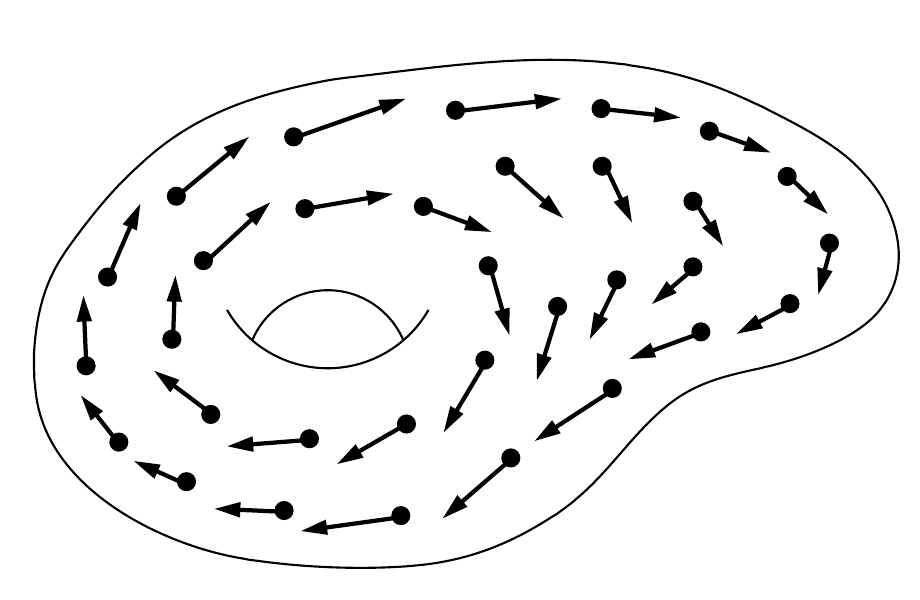
\includegraphics[scale=0.25]{Figuras/CampoVectorial.png}
				\caption{Campo vectorial suave}
			\end{figure}
		}

		\only<2>{ \begin{align*}
				g_p(-,-)               : & T_{p}M \times T_{p}M \to \mathbb{R} \\[10pt]
				g_p(\lambda x + y, z)    & = \lambda g_p(x,z) + g_p(y,z)       \\
				g_p(x,\lambda y + z)     & = \lambda g_p(x,y) + g_p(x,z)       \\
			\end{align*} }
		\only<3>{\[
				g_p(x,y) = g_p(y,x)
			\]}
		\only<4>{\begin{align*}
				g_{p}(x,x) & > 0, \quad \text{ si } x \neq 0 \\
				g_{p}(0,0) & = 0, \quad \text{ si } x = 0
			\end{align*} }

		\only<5> {
			\begin{figure}[t]
				\scalebox{0.75}{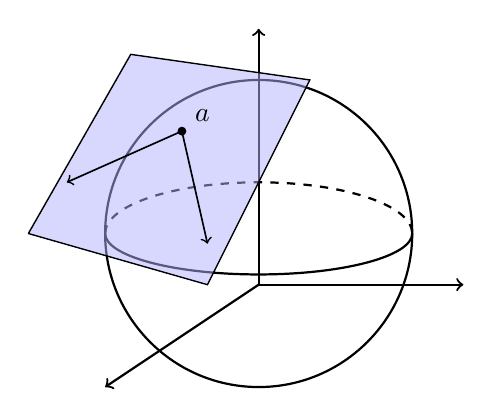
\begin{tikzpicture}[scale=0.65]
	% Esfera
	\draw [thick] (3,0) arc (0:180:3 and -0.8);
	\draw [thick, dashed] (-3,0) arc (180:0:3 and 1);
	\draw [thick] (0,0) circle (3);

	% Ejes R3
	\draw [thick,->] (0,-1) -- (0,4);
	\draw [thick,->] (0,-1) -- (4,-1);
	\draw [thick,->] (0,-1) -- (-3,-3);


	% Rectángulo (Espacio Tangente)
	\draw [fill=blue!30!white,opacity=0.5, line width=0] (-4.5,0) -- (-2.5,3.5) --(1,3.0) -- (-1,-1) -- (-4.5,0);
	\draw [line width=0.5] (-4.5,0) -- (-2.5,3.5) --(1,3.0) -- (-1,-1) -- (-4.5,0);
	\filldraw (-1.5,2) circle (0.075);
	\node at (-1.1,2.3) {$a$};


	\draw [semithick, ->] (-1.5,2) -- (-1,-0.2);
	\draw [semithick, ->] (-1.5,2) -- (-3.75,1);
\end{tikzpicture}
}
			\end{figure}
		}
	\end{columns}

	\vspace{24pt}

	\only<5>{ En pocas palabras, una métrica Riemanniana define un producto interno en el espacio tangente a cada punto de una variedad suave.}
	\only<6> {\begin{definition}[Variedad Riemanniana]
			El par $(M,g)$, donde $M$ es una variedad suave y $g$ es una métrica Riemanniana, es llamado un \textbf{Variedad Riemanniana}. \end{definition} }
\end{frame}

\begin{frame}
	\frametitle{Variedades Riemannianas}
	\begin{lemma}[Expresión local de la métrica]
		\label{Lemma: Expresión local de la métrica}
		Sean $(M,g)$ una variedad Riemanniana, $p \in M$ y $(U,\phi)$ una carta suave que contiene a $p$. La métrica puede expresarse de manera local en $U$ como:
		\[
			g = \sum_{i=1}^{n}\sum_{j=1}^{n} g_{ij} d\phi_i d\phi_j,
		\]
		donde $\{ d\phi_{1}, \ldots, d\phi_{n} \}$ es la base del espacio dual a $T_{p}M$, asociada a la base $\{ \partial \phi_{1}, \ldots, \partial \phi_{n} \}$, y $g_{ij}$ son funciones suaves dadas por:
		\[
			g_{ij}(p) = g_{p}\left( \partial \phi_{i} \big|_{p}, \partial \phi_j \big|_{p}\right)
		\]
	\end{lemma}
\end{frame}

\begin{frame}
	\frametitle{Variedades Riemannianas}
	Dada una métrica $g$ es posible asociar a esta una matriz $G$, la cual depende de las coordenadas locales de la carta sobre la cual esté definida. \pause Las entradas de $G$ son las funciones $g_{ij}$ definidas anteriormente.
	\[
		G = \begin{bmatrix}
			g_{11} & g_{12} & \cdots & g_{1n} \\
			g_{21} & g_{22} & \cdots & g_{2n} \\
			\vdots & \vdots & \ddots & \vdots \\
			g_{n1} & g_{n2} & \cdots & g_{nn}
		\end{bmatrix}
	\]\pause

	\vspace{12pt}

	La matriz $G$ es simétrica y definida positiva.
\end{frame}


\begin{frame}
	\frametitle{Métrica Euclidiana}\pause
	\begin{example}
		En $\mathbb{R}^{n}$ con la base estándar $\{x_{1}, \ldots, x_{n}\}$ definimos la métrica:
		\[
			g = \sum_{i=1}^{n} \sum_{j=1}^{n} \delta_{ij} dx_{i} dx_{j} = \sum_{i=1}^{n} \left(dx_{i}\right)^{2}
			\only<3>{, \quad G = I_{n \times n}}
		\] \pause \pause
		Aplicando esta métrica a dos vectores tangentes arbitrarios $v = \begin{bmatrix} v_1 \cdots v_n \end{bmatrix}$ y $w = \begin{bmatrix} w_1 \cdots w_n \end{bmatrix}$ se obtiene:
		\begin{align*}
			g(v,w) & = \sum_{i=1}^{n} dx_{i}(v) dx_{i}(w)   \\
			       & = \sum_{i=1}^{n}v_{i}w_{i} = v \cdot w
		\end{align*}
	\end{example}
\end{frame}

\begin{frame}
	\frametitle{Variedades Riemannianas}\pause
	\begin{theorem}[Existencia de la métrica] Toda variedad suave puede ser equipada con una métrica Riemanniana.
	\end{theorem}\pause
	\begin{proof}
		\begin{enumerate}
			\item Sea $M$ una variedad suave y $(U_{\alpha},\phi_{\alpha})$ cualquier carta suave en $M$. \pause
			\item Dado un punto $p$ en la carta $(U_\alpha,\phi_\alpha)$ y dos vectores tangentes $v,w$ en $T_{p}M$ como, podemos expresar a estos como una combinación lineal:
			      \[
				      v = \sum_{i=1}^{n} v_{i} \partial \phi_{i}, \quad
				      w = \sum_{j=1}^{n} w_{j} \partial \phi_{j},
			      \]
		\end{enumerate}
	\end{proof}
\end{frame}

\begin{frame}
	\begin{proof}
		\begin{enumerate}
			\setcounter{enumi}{2}
			\item Definimos en $U_{\alpha}$ la métrica $g^{\alpha}$ como:
			      \[
				      g_{p}^{\alpha}(v,w) = \sum_{i=1}^{n}\sum_{j=1}^{n} \delta_{ij} v_{i}w_{j} = \sum_{i=1}^{n} v_{i} w_{i}
			      \] \pause
			\item Utilizando una partición de la unidad $\{f_{\alpha}\}$ subordinada a la estructura suave de $M$ se construye una métrica global $g$, de tal modo que:
			      \[
				      g_p = \sum_{\alpha} f_{\alpha} g_{p}^{\alpha}
			      \]
		\end{enumerate}
	\end{proof}
\end{frame}

\begin{frame}
	\begin{figure}[t]
		\scalebox{0.75}{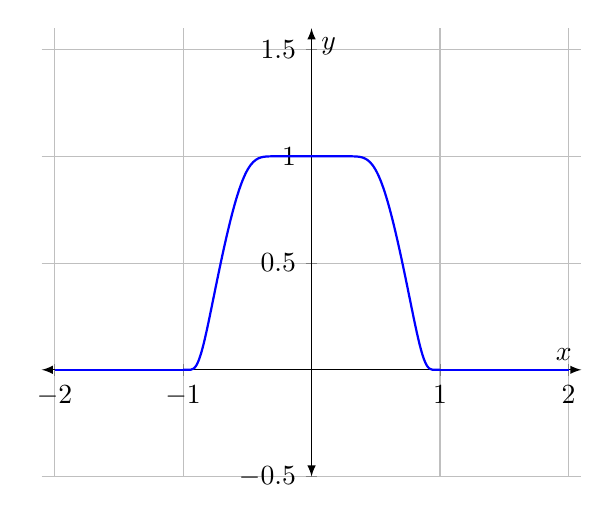
\begin{tikzpicture}
\begin{axis}[
  grid=both,
  xmin=-2.1,
  xmax=2.1,
  ymin=-0.5,
  ymax=1.6,
  axis lines=middle,
  xlabel = $x$,
  ylabel = $y$,
  axis line style={latex-latex},
  ]

\addplot[
  samples=100,
  domain=-1:1,
  color=blue,
  thick,
  smooth,
  ]
  {1 -( ((e)^(-1/(x^2))) / ( ( e^(-1/(x^2)) ) + (e^(-1/(1-(x^2)))) ))};


\addplot[
  samples=2,
  domain=-2:-0.99,
  color=blue,
  thick,
  smooth
  ]
  {0};

\addplot[
  samples=2,
  domain=0.99:2,
  color=blue,
  thick,
  smooth
  ]
  {0};
\end{axis}
\end{tikzpicture}
}
		\caption{Gráfica de una función indicadora suave.}
	\end{figure}
\end{frame}

\begin{frame}
	\frametitle{Curvas en Variedades}
	\begin{definition}[Curva en variedades]
		Sea $M$ una variedad suave, diremos que $\gamma$ es \textbf{una curva suave} sobre $M$ si $\gamma: [a,b] \to M$ es un mapa suave.
	\end{definition} \pause

	\begin{definition}[Velocidad de una curva]
		Sean $\gamma: [a,b] \to M$ una curva suave, $t_0 \in [a,b]$ y $(U,\phi)$ una carta suave que contiene a $\gamma(t_0)$. Definimos la \textbf{velocidad de $\gamma$ en $t_0$} como el vector tangente:
		\[
			\gamma'(t_0) = \sum_{i=1}^{n} \frac{d\gamma_i(t_0)}{dt} \partial \phi_{i} \big|_{\gamma(t_0)}
		\]
	\end{definition}
\end{frame}

\begin{frame}
	\frametitle{Curvas en Variedades}
	\begin{figure}
		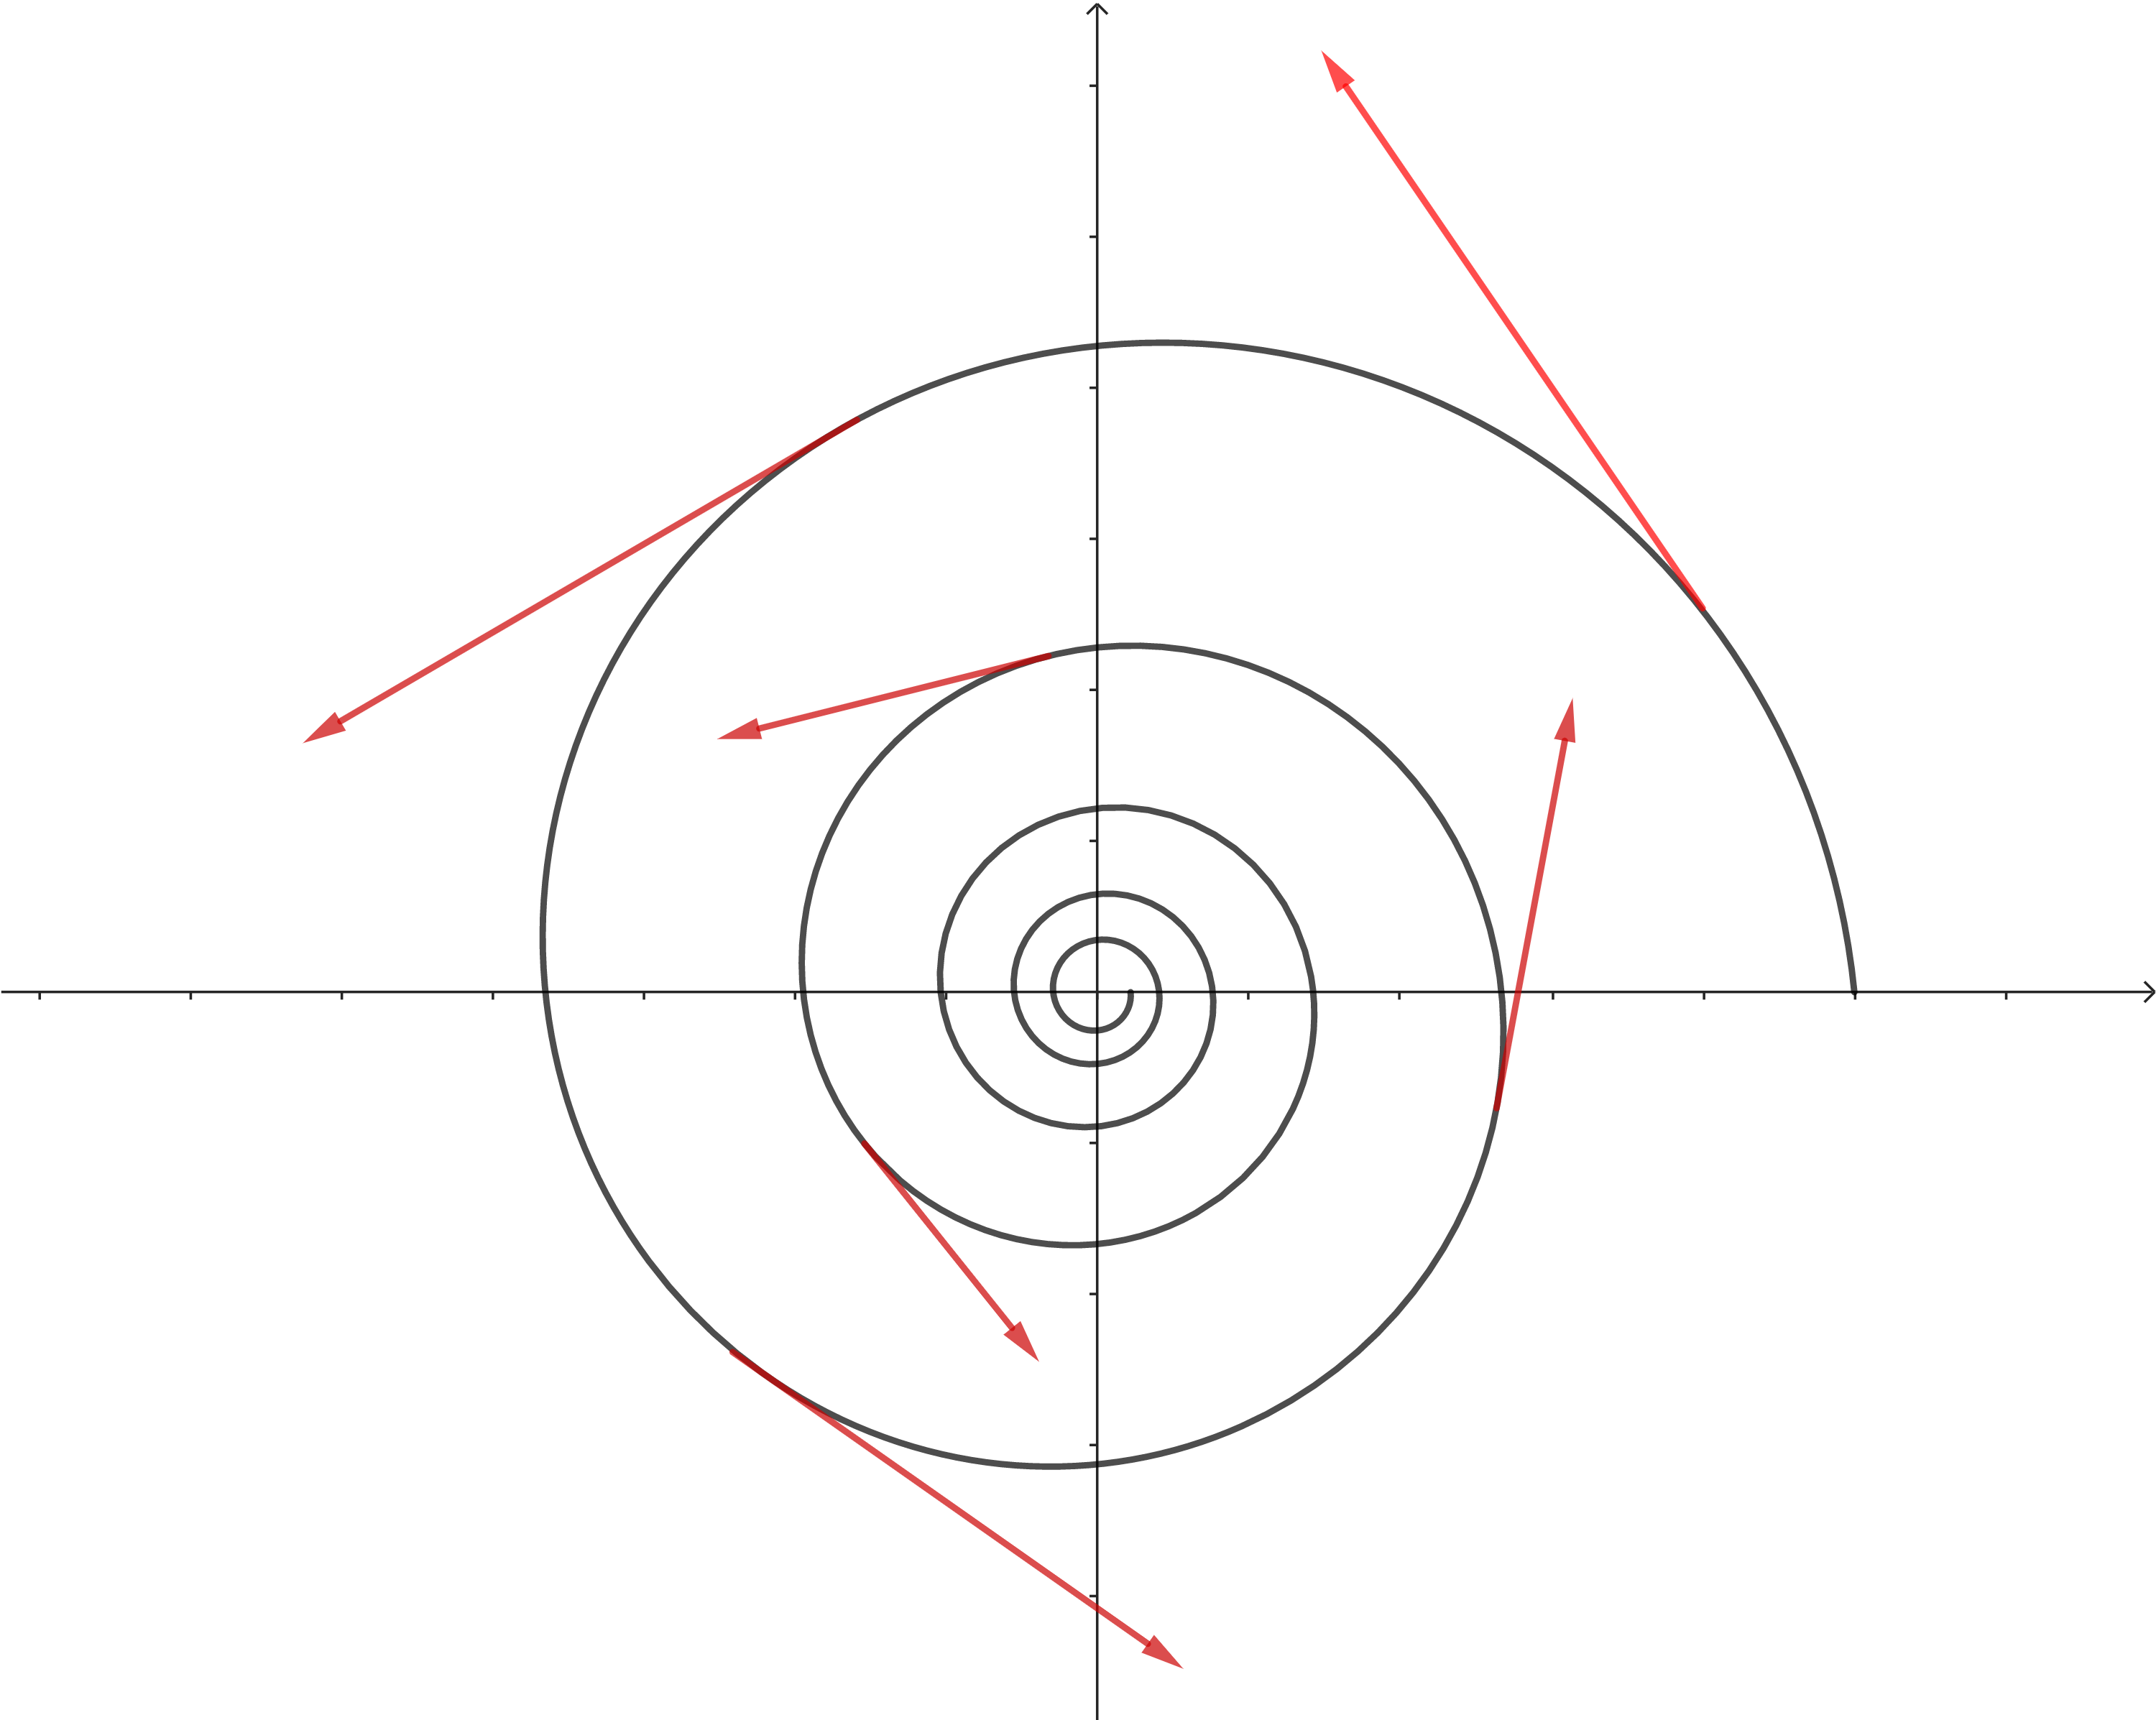
\includegraphics[scale=2.5]{Figuras/CurvaLogaritmica.png}
		\caption{Ejemplo de una curva en el plano con algunos vectores tangentes.}
	\end{figure}
\end{frame}

\begin{frame}
	\frametitle{Conexión Afín}
	\begin{definition}[Conexión afín]
		Una \textbf{conexión afín} en $M$ es un mapa bilineal:
		\[
			\nabla: \mathfrak{X}(M) \times \mathfrak{X}(M) \to \mathfrak{X}(M),
		\]\pause
		el cual cumple las siguientes dos propiedades:
		\begin{itemize}
			\item $\nabla$ es lineal en su primera coordenada con respecto al anillo de funciones suaves.
			      \[
				      \nabla(fX + Y, Z) = f\nabla(X,Z) + \nabla(Y,Z)
			      \]\pause
			\item $\nabla$ cumple la siguiente regla del producto:
			      \[
				      \nabla(X,fY) = X(f) Y + f\nabla(X,Y)
			      \]
		\end{itemize}
	\end{definition}
\end{frame}


\begin{frame}
\begin{center}
	\begin{figure}[h]
		\centering
		\begin{subfigure}{0.30\textwidth}
			\centering
			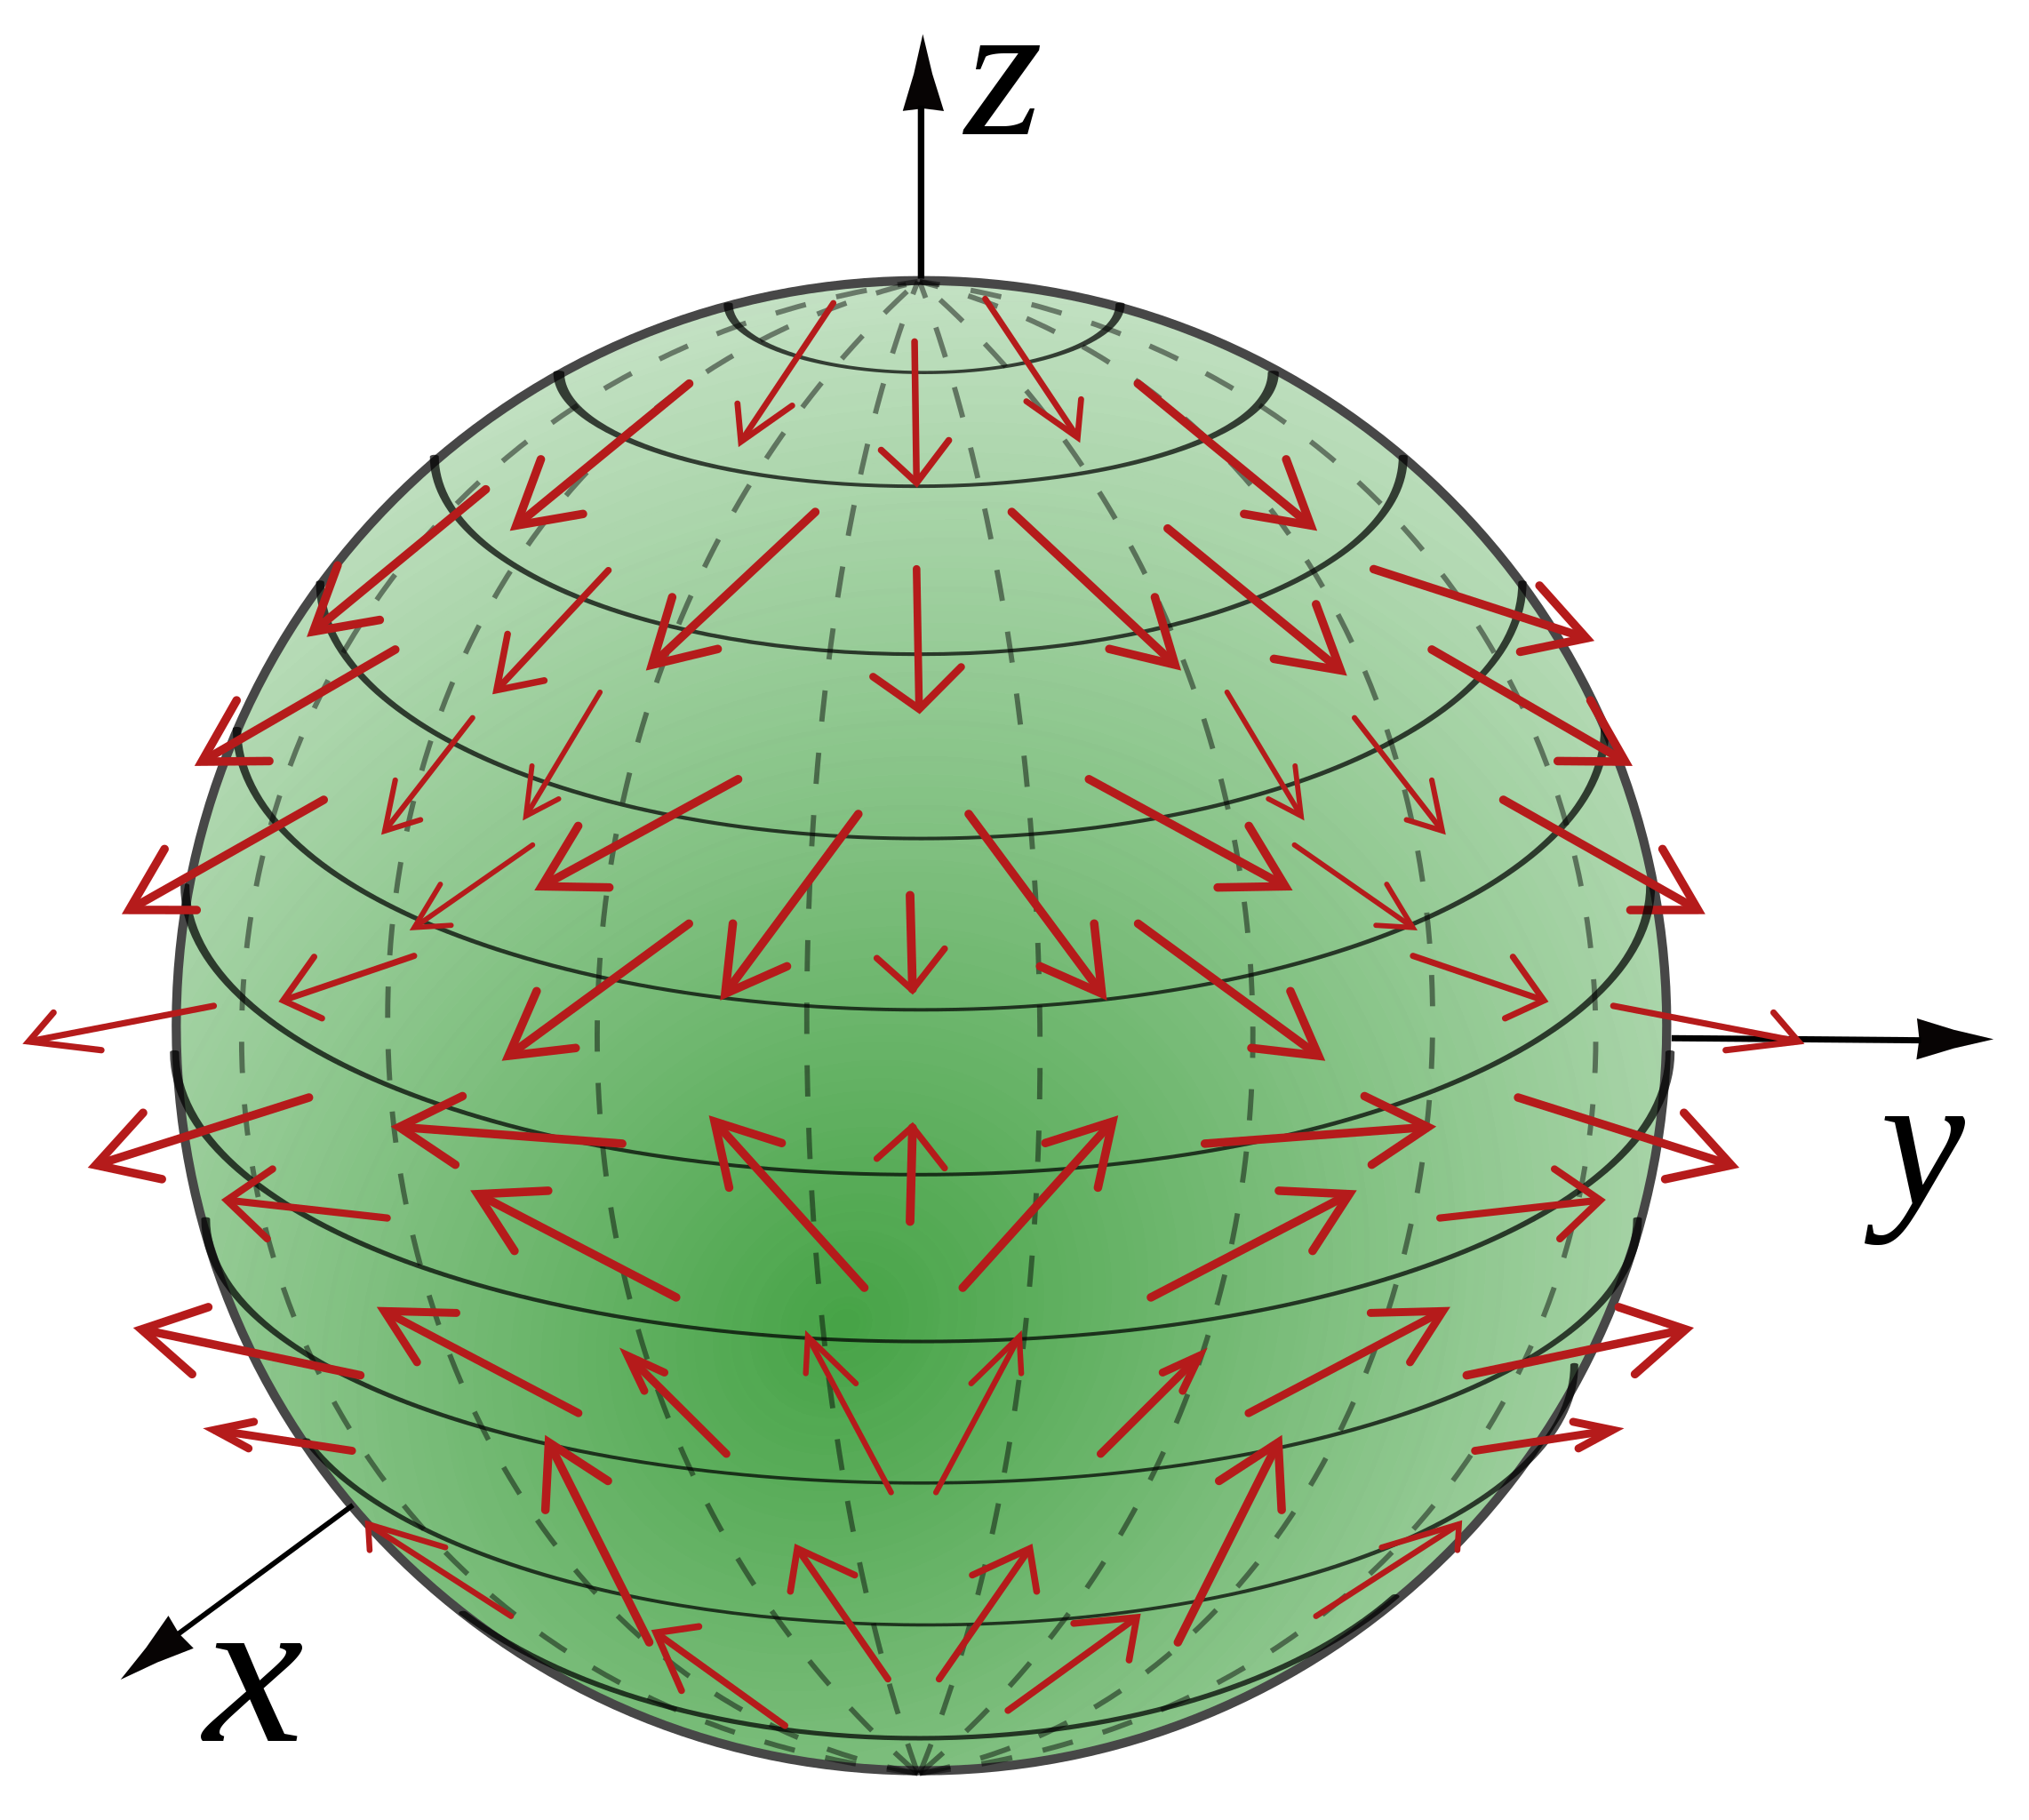
\includegraphics[scale=0.065]{Figuras/Vector_sphere.svg.png}
		\end{subfigure}
		\hspace{50pt}
		\begin{subfigure}{0.30\textwidth}
			\centering
			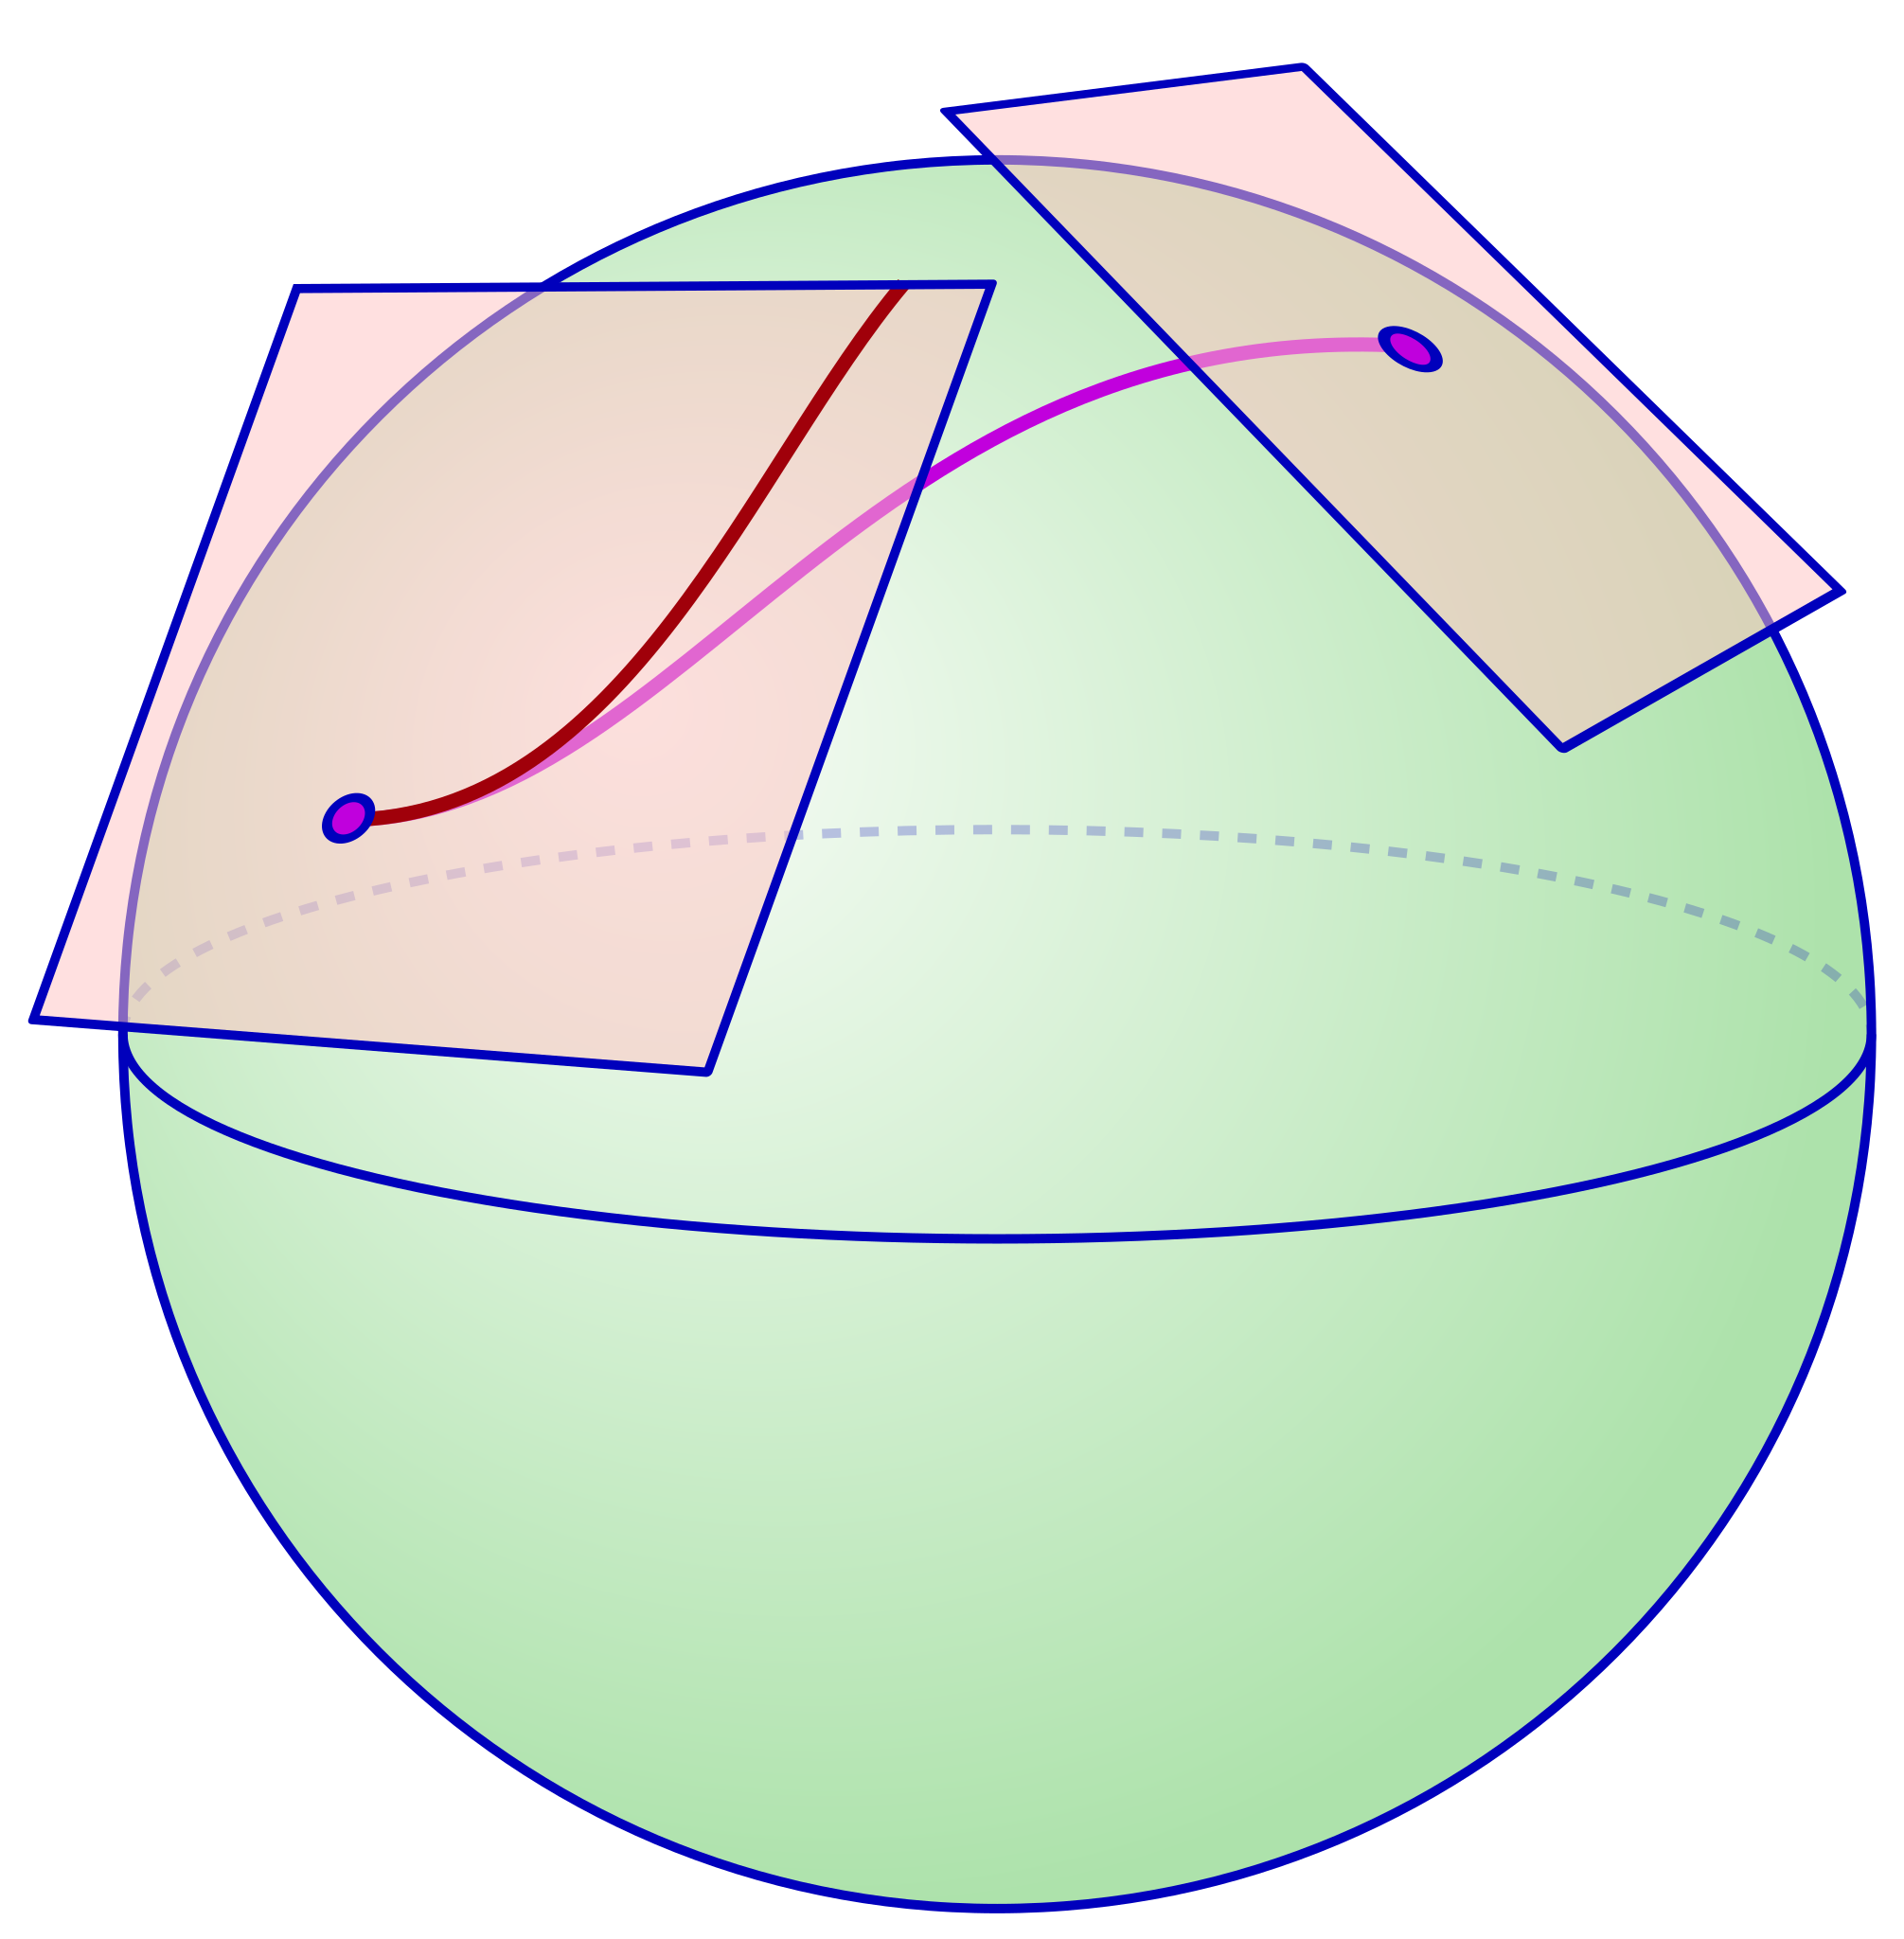
\includegraphics[scale=0.065]{Figuras/TransporteParalelo.png}
		\end{subfigure}
		\caption{Representación de una conexión afín en la esfera}
	\end{figure}
\end{center}
\end{frame}

\begin{frame}
	\frametitle{Conexión Afín}
	Usualmente se denota a la conexión afín $\nabla(X,Y)$ como $\nabla_{X}Y$ y se le llama \textit{la derivada covariante de $Y$ en la dirección de $X$}.

	\pause

	\vspace{12pt}

	De manera local la derivada covariante puede ser expresada como:
	\[
		\nabla_{X}Y = \sum_{k=1}^{n} \left(
		X(Y_{k}) + \sum_{i=1}^{n}\sum_{j=1}^{n} \Gamma_{ij}^{k} X_{i}Y_{j}
		\right) \partial_{k},
	\]\pause
	En la ecuación anterior $\Gamma_{ij}^{k}$ son $n^{3}$ funciones suaves, a las cuales se les llama los \textit{símbolos de Christoffel}. \pause En una variedad Riemanniana los símbolos pueden ser obtenidos por la ecuación:
	\[
		\Gamma_{ij}^{m} = \frac{1}{2} \sum_{k=1}^{n} (\partial_{i} g_{jk} + \partial_{j}g_{ji} - \partial_{k}g_{ij}) g^{km}
	\]
\end{frame}

\section{Geodésicas}

\begin{frame}
	\frametitle{Geodésicas}
	\begin{definition}
		Sea $M$ una variedad suave equipada con una conexión afín $\nabla$. Diremos que una curva $\gamma: [a,b] \to M$ es una \textbf{curva geodésica} si:
		\[
			\nabla_{\gamma'(t)} \gamma'(t) = 0
		\]
	\end{definition}
\end{frame}

\begin{frame}
	\frametitle{Existencia y unicidad de geodésicas}
	\begin{theorem}
		Sea $M$ una variedad suave equipada con una conexión afín. Para cada punto $p \in M$, cada vector tangente $v \in T_{p}M$ y cada real $t_0$ existe un intervalo abierto $I \subset \mathbb{R} $ que contiene a $t_0$ y una geodésica $\gamma(t) : I \to M $ que satisface $\gamma(t_0) = p$ y $\gamma'(t_0) = v$. \pause Cualesquiera dos geodésicas que satisfagan las mismas condiciones coincidirán en la intersección de sus dominios.
	\end{theorem}

\end{frame}

\begin{frame}
	\frametitle{Existencia y unicidad de geodésicas}
	\begin{proof}
		\begin{enumerate}
			\item Como se mencionó anteriormente, dada una carta $(U,\phi)$ se puede expresar a la conexión en términos de las coordenadas locales como:
			      \[
				      \nabla_{\gamma'(t)}\gamma'(t) = \sum_{k=1}^{n} \left(
				      \frac{d\gamma'_k(t)}{dt} + \sum_{i=1}^{n}\sum_{j=1}^{n} \frac{d\gamma_{i}(t)}{dt} \Gamma_{ij}^{k}\gamma_{j}'(t)
				      \right) \partial_{k}			      \] \pause
			\item Por definición de geodésica, $\nabla_{\gamma'(t)}\gamma'(t) = 0$, esto ocurre si y solo si:
			      \[
				      \gamma''_{k}(t) + \sum_{i=1}^{n}\sum_{j=1}^{n} \Gamma_{ij}^{k}\gamma_{i}'(t) \gamma_{j}'(t) = 0
			      \]
		\end{enumerate}
	\end{proof}
\end{frame}

\begin{frame}
	\frametitle{Existencia y unicidad de geodésicas}
	\begin{proof}
		\begin{enumerate}
			\setcounter{enumi}{2}
		\item Esta ecuación, a la cual se le llama la \textbf{ecuación geodésica}, puede ser reducida realizando la sustitución $\gamma''(t) = x'(t)$, de modo que obtenemos:
			      \[
				      x_{k}'(t) + \sum_{i=1}^{n} \sum_{j=1}^{n} \Gamma_{ij}^{k} x_{i}(t) x_{j}(t) = 0.
			      \] \pause
			\item El teorema de existencia y unicidad de las ecuaciones diferenciales ordinarias garantiza que este sistema tendrá solución y dicha solución será única.
		\end{enumerate}
	\end{proof}
\end{frame}

\begin{frame}
	\frametitle{Geodésicas en $\mathbb{H}^2$}
	\begin{definition}[Espacio hiperbólico de dimensión $2$]
		Consideremos al subconjunto de $\mathbb{R}^{2}$:
		\[
			\mathbb{H}^{2} = \{(x,y) : x \in \mathbb{R}, y > 0\},
		\]\pause
		este subconjunto es un abierto en $\mathbb{R}^{2}$, por lo cual es una variedad topológica, este subconjunto puede ser cubierto por una única carta, por lo cual está determina una estructura suave. \pause Hacemos de $\mathbb{H}^{2}$ una variedad Riemanniana dotándolo de la métrica cuyos coeficientes son:
		\[
			g_{ij} = \frac{R \delta_{ij}}{y^{2}}, \quad R \in \mathbb{R}
		\]\pause
		a esta variedad Riemanniana se le conoce como \textbf{espacio hiperbólico de dimensión 2} o \textbf{modelo de Poincaré del semiplano superior}.
	\end{definition}
\end{frame}

\begin{frame}
	\frametitle{Geodésicas en $\mathbb{H}^2$}
	Para calcular las geodésicas en el $\mathbb{H}^{2}$ comenzamos calculando los símbolos de Christoffel. \pause
	\[
		\Gamma_{ij}^{m} = \frac{1}{2} \sum_{k=1}^{2}(\partial_{i} g_{jk} + \partial_{j} g_{ki} - \partial_{k}g_{ij})g^{km}
	\]\pause

	\begin{columns}[t]
		\column{.1\textwidth}
		\begin{align*}
			\Gamma_{11}^{1} & = 0           \\[12pt]
			\Gamma_{11}^{2} & = \frac{1}{y}
		\end{align*}
		\column{.1\textwidth}
		\begin{align*}
			\Gamma_{12}^{1} & = -\frac{1}{y} \\[12pt]
			\Gamma_{21}^{1} & = -\frac{1}{y}
		\end{align*}
		\column{.1\textwidth}
		\begin{align*}
			\Gamma_{12}^{2} & = 0 \\[24pt]
			\Gamma_{21}^{2} & = 0
		\end{align*}
		\column{.1\textwidth}
		\begin{align*}
			\Gamma_{22}^{1} & = 0            \\[12pt]
			\Gamma_{22}^{2} & = -\frac{1}{y}
		\end{align*}
	\end{columns}
\end{frame}

\begin{frame}
	\frametitle{Geodésicas en $\mathbb{H}^2$}
	Si $\gamma$ es una curva podemos suponer que está parametrizada como $\gamma(t) = (x(t),y(t))$, \pause si $\gamma(t)$ es una curva geodésica al sustituir estas parametrizaciones y los símbolos de Christoffel en la ecuación geodésica obtendremos el sistema de ecuaciones diferenciales:
	\[
		\begin{cases}
			x'' - \frac{2}{y} x'y'                         & = 0 \\[12pt]
			y'' + \frac{1}{y} (x')^2 - \frac{1}{y}(y')^{2} & = 0
		\end{cases}
	\] \pause

	Las soluciones de este sistema de ecuaciones son las siguientes:
	\vspace{12pt}
	\begin{columns}
		\column{0.4\textwidth}
		\centering
		Si $x'(t) = 0$, \\[12pt]
		$y = y_{0}e^{kt}$
		\column{0.4\textwidth} \pause
		\centering
		Si $x'(t) \neq 0$, \\[12pt]
		$(x - C)^{2} + y^{2} = \frac{k_0}{K_{1}^{2}}$
	\end{columns}
\end{frame}

\begin{frame}
	\frametitle{Geodésicas en $\mathbb{H}^2$}
	\begin{figure}[h]
		\centering
		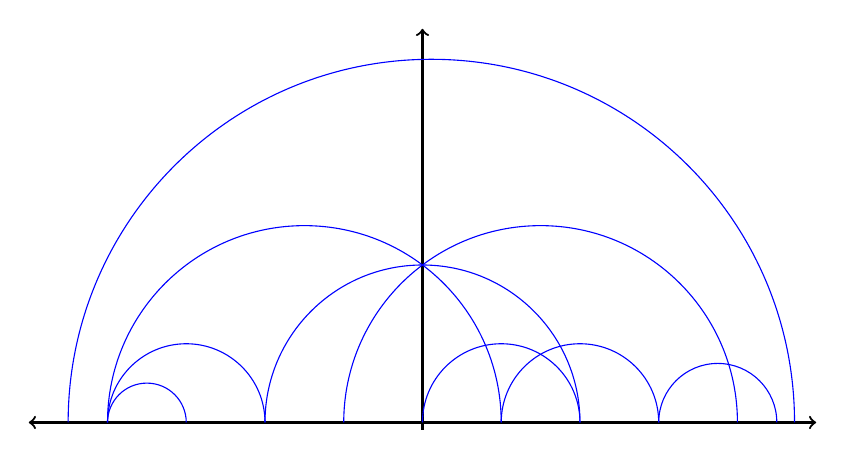
\begin{tikzpicture}
  \draw[color=black,thick,<->] (-5,0) -- (5,0);
  \draw[color=black,thick,<-] (0,5) -- (0,-0.1);

  \draw[blue] (2,0) arc (0:180:1);
  \draw[blue] (2,0) arc (0:180:2);
  \draw[blue] (3,0) arc (0:180:1);
  \draw[blue] (3,0) arc (180:0:0.75);
  \draw[blue] (-1,0) arc (180:0:2.5);
  \draw[blue] (-4,0) arc (180:0:2.5);
  \draw[blue] (-4,0) arc (180:0:0.5);
  \draw[blue] (-4,0) arc (180:0:1);
  \draw[blue] (-4.5,0) arc (180:0:4.6125);
\end{tikzpicture}

		\caption{Representación de algunas geodésicas en $\mathbb{H}^{2}$}
	\end{figure}
\end{frame}

\section{Conclusiones}
\begin{frame}
	\frametitle{Conclusiones}
	\begin{enumerate}
		\item En este trabajo se desarrollaron herramientas de la teoría de variedades suaves. Se estudiaron las propiedades de las variedades topológicas y las variedades suaves. \pause
		\item Se trasladaron conceptos del cálculo en espacios euclidianos a las variedades suaves. \pause
		\item Se trabajaron conceptos de geometría Riemanniana. \pause
			\begin{itemize}
				\item Se definieron conceptos como las métricas Riemannianas, las conexiones y las curvas geodésicas. \pause
				\item Se demostró la existencia de las métricas en variedades suaves, así como la existencia y unicidad de las conexiones y las geodésicas. \pause
			\end{itemize}
		\item Se definió el espacio hiperbólico de dimensión $2$ y se encontraron las curvas geodésicas.
	\end{enumerate}
\end{frame}



\begin{frame}[allowframebreaks]
\frametitle{Referencias}
\nocite{lee2013introduction}
\nocite{tu2010introduction}
\nocite{spivak1971calculus}
\nocite{duistermaat2004multidimensional}
\nocite{lee2009manifolds}
\nocite{warner2013foundations}
\nocite{greub2012multilinear}
\nocite{hoffman2015linear}
\nocite{rudin1976principles}
\nocite{gopalakrishnan1984commutative}
\nocite{munkres2000topology}
\nocite{roman2007advanced}
\nocite{lee2019introduction}
\nocite{tao_2016}
\nocite{whitney1936differentiable}
\nocite{tu2017differential}
\nocite{delia2011geodesia}
\nocite{do1992riemannian}
\nocite{biezuner2020geometry}

\printbibliography
\end{frame}


\end{document}
